\apendice{Especificación de diseño}

\section{Introducción}

En este anexo se introducirá el diseño de los distintos aspectos de este proyecto a todos los niveles \textit{software}.

\section{Diseño de datos}

En este trabajo se manejan dos tipos de datos principales:

\begin{itemize}
	\item Imágenes con formato JPG.
	\item Ficheros JSON que contienen las coordenadas de las etiquetas realizadas con el etiquetador de imágenes.
\end{itemize}

Tanto las imágenes como las etiquetas de las imágenes se almacenan de manera persistente en el almacenamiento de nuestro disco duro. Para observarlas deberemos seguir dentro del proyecto la siguiente ruta de carpetas: \textit{code}, \textit{rsc}, \textit{img}. Una vez situados en la carpeta \textit{img}, nos encontraremos una serie de carpetas con el nombre de cada tipo de fitolito y una carpeta \textit{Default}\footnote{Siempre y cuando hayamos utilizado el etiquetador anteriormente.}.% Aclarar
% Añadir captura de pantalla: tanto de carpetas

La razón de la existencia de una carpeta por cada tipo de fitolito es el almacenamiento organizado de los recortes generados por cada etiqueta realizada con el etiquetador. Almacenando en cada una de estas carpetas los recortes correspondientes a un tipo de fitolito. 

Respecto a la carpeta Default, en ella se almacenan las imágenes completas junto a un fichero \textit{JSON} por imagen. En cada uno de estos ficheros se almacenan las coordenadas  realizadas con el etiquetador en dicha imagen. Un ejemplo del contenido de un fichero JSON sería el siguiente:

\begin{verbatim}
{"2017_5_17_17_57Image_7344.jpg": 
	{"Bilobate": [[865, 1110, 1183, 1402]], 
		"Spherical": [[1132, 1282, 2207, 2357], [1238, 1414, 368, 533]]}}
\end{verbatim}

Siendo el formato: nombre de la imagen y nombre de cada tipo de fitolito, solo apareciendo los existentes en la imagen. Teniendo cada tipo de fitolito una lista de etiquetas, donde cada etiqueta tiene 4 coordenadas. Por último, las 4 coordenadas de cada etiqueta se almacenan con el siguiente formato y orden:

\begin{itemize}
	\item Desplazamiento en el eje y de la esquina superior izquierda de una etiqueta.
	\item  Desplazamiento en el eje y de la esquina inferior derecha de una etiqueta.
	\item Desplazamiento en el eje x de la esquina superior izquierda de una etiqueta.
	\item  Desplazamiento en el eje x de la esquina inferior derecha de una etiqueta.
\end{itemize}
%Captura

\section{Diseño procedimental}

En este proyecto hay que destacar tres procedimientos principales, los cuales explicaré ,brevemente, a continuación.

\begin{comment}
\begin{itemize}
	\item Procedimiento que realiza el etiquetador de imágenes.
	\item Procedimiento en el \textit{notebook} para la detección de caras.
	\item Procedimiento de entrenamiento de \textit{YOLO}.
\end{itemize}
\end{comment}

\subsection{Procedimiento que realiza el etiquetador de imágenes}

El procedimiento muy simplificado del funcionamiento del etiquetador cuando se carga una nueva imagen es el mostrado en el procedimiento \ref{alg:1}.

\begin{algorithm}
    \If{Cambio de imagen}
    	{
    	Cargamos imagen.
    	
    	\If{La imagen se encuentra en el directorio por defecto y tiene un fichero JSON correspondiente}
    		{
    			Cargamos las etiquetas previamente realizadas.
    			
    			Mostramos las etiquetas junto a la imagen.
    		}
    	Escuchamos los eventos del ratón sobre el SVG.
    	}
    \caption{Procedimiento de funcionamiento del etiquetador}
    \label{alg:1}
\end{algorithm}

Una vez cargada la imagen, como indico finalmente, se escuchan los eventos del ratón. En concreto, los \textit{clicks} y movimientos de este sobre el SVG. Ya que la creación de los rectangulos, o etiquetas, sobre la imagen se hacen a partir de dichos eventos. Para ello, se poseen dos \textit{listeners}, u observadores de eventos, uno para cada evento. Los \textit{clicks} se utilizan para la creación de un nuevo rectángulo o su finalización. Y los movimientos del ratón, una vez hecho un primer click\footnote{De manera que hayamos creado el rectángulo}, permiten redimensionar el rectángulo de manera totalmente intuitiva.

Nótese que existen más variables a tener en cuenta, como el tipo de fitolito, el cual determina el directorio donde se guardará el recorte obtenido de la etiqueta y como se almacenan las coordenadas en el fichero \textit{JSON}, entre otras. Pero lo que se intenta realizar en este apartado es una introducción simplificada del procedimiento.

\subsection{Procedimiento en el \textit{notebook} para la detección de caras}

El procedimiento simplificado del funcionamiento del \textit{notebook} para el reconocimiento de caras en una imagen es el mostrado en el procedimiento \ref{alg:2}.

%COMPLETAR
\begin{algorithm}
    Realizamos la ventana deslizante sobre la imagen.
    
    Obtenemos las características del histograma de los gradientes.

    Eliminamos las ventanas redundantes con non-maximum suppression.

    Mostramos la imagen con los rectangulos.
    \caption{Procedimiento de funcionamiento del etiquetador}
    \label{alg:2}
\end{algorithm}

\subsection{Procedimiento de entrenamiento de \textit{YOLO}}

Para realizar el entrenamiento de \textit{YOLO}, \textit{darkflow} nos provee de un \textit{script} que nos facilita dicha tarea, llamado \textit{flow}. Además, existen dos posibilidades principalmente para realizar el entrenamiento sobre nuestro \textit{dataset}:

\begin{itemize}
	\item Utilizar unos pesos\footnote{Pesos: son cada uno de los valores asignados a una neurona en una red neuronal.} entrenados para nuestro modelo.
	\item Crear un modelo que se ajuste a nuestras necesidades.
\end{itemize}

La ventaja de utilizar unos pesos pre-entrenados reside en que la red neuronal ya habrá aprendido ciertas características, como bordes o formas. Por lo tanto, el tiempo de entrenamiento será mucho menor. Pero puede que la reutilización de dicho modelo no se adecue a nuestras necesidades ya sea porque tengamos un número distinto de clases al modelo inicial o porque el contexto sea totalmente distinto.

Por otro lado, se encuentra el entrenamiento desde cero de un nuevo modelo que se adecue a nuestras necesidades. El cual suple las desventajas presentadas por la anterior opción, pero introduce una mayor complejidad a la hora del entrenamiento.

En cualquier caso, los dos siguientes ejemplos, correspondientes a las opciones planteadas, nos permitirían entrenar el modelo:

\begin{verbatim}
flow --train --model cfg/yolo-tiny.cfg
 --load bin/yolo-tiny.weights
 --dataset "Fitolitos" --annotation "Fitolitos"

or

flow --model cfg/yolo-new.cfg --train
 --dataset "Fitolitos" --annotation "Fitolitos"
\end{verbatim}

Donde la opción \textit{--train} indica que se desea entrenar un modelo, la opción \textit{--load} indica donde se encuentran los pesos pre-entrenados, la opción \textit{--dataset} indica la ruta de la carpeta donde se encuentran las imagenes de los fitolitos y la opción \textit{--annotation} indica donde se encuentran los ficheros con las coordenadas\footnote{La modificaciones realizadas sobre \textit{darkflow} para permitir la lectura y conversión de mis coordenadas están pensados para que el valor de las opciones \textit{dataset} y \textit{annotation} sean el mismo. De otra manera el modelo fallará en el entrenamiento.}. 

\section{Diseño arquitectónico}

Este proyecto no contiene un diseño muy elaborado a nivel arquitectónico por dos razones fundamentales. La primera ha sido el esfuerzo requerido en la investigación y aprendizaje por mi parte de técnicas muy variadas para afrontar el problema. Hasta llegar con la más adecuada. Por otro lado, la mayoría del código ha sido desarrollado en los \textit{Jupyter Notebooks}. Los cuales nos permiten interaccionar fácilmente con el código y documentarlo a su vez, aportando una fácil introducción a otros usuarios.

Aun así existen dos módulos con código empaquetado: módulo utilizado por el \textit{notebook} para la predicción de caras y módulo utilizado para la gestión de carpetas del etiquetador. Véase COMPLETAR REF.



Por un lado, tenemos el módulo que se encarga de la gestión de carpetas. Con los siguientes métodos y atributos.

Y, por otro lado, tenemos las clases encargadas de la predicción de una nueva imagen mediante el \textit{notebook} citado anteriormente.



\section{Diseño de las interfaces}

En esta sección se explicarán las diferentes interfaces de los productos realizados en este trabajo fin de grado.

\subsection{\textit{Jupyter Notebook} para la detección de caras}

Durante el primer mes se trabajo en un \textit{Jupyter Notebook} que trataba de reconocer caras mediante un clasificador junto a un extractor de características, como ya hemos explicado en secciones anteriores. Con este \textit{Jupyter Notebook} se trataba de facilitar la evaluación del rendimiento de los clasificadores y el cambio de las distintas variables de manera interactiva. 

Por lo tanto, la interfaz de este \textit{Jupyter Notebook} no ha sido trabajada para su uso por parte del usuario. Sino que fue creada para un uso más de experimentación. Es por ello que la interfaz no tiene un buen grado de usabilidad como podemos observar en la figura \ref{fig:C.5.1}.

\begin{figure}[h]
\centering
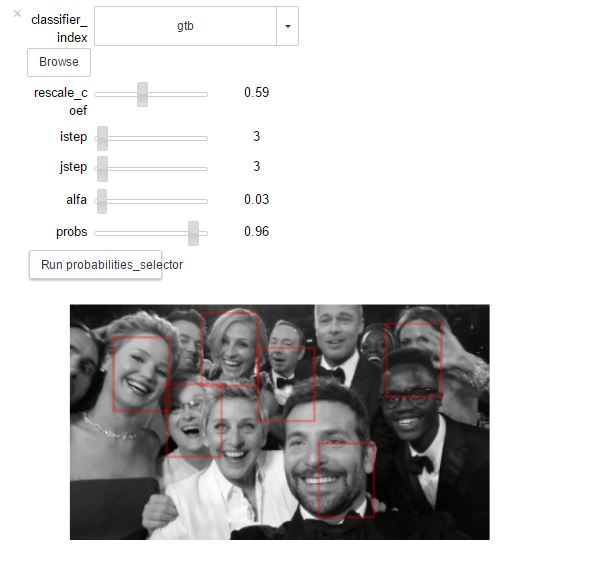
\includegraphics[width=0.99\textwidth]{reconocimiento_de_caras_notebook_v1}
\caption{\textit{Jupyter Notebook} para el reconomiento de caras}
\label{fig:C.5.1}
\end{figure}

\subsection{Etiquetador de imágenes}

La interfaz del etiquetador de imágenes ha sido desarrollada partiendo del prototipo mostrado en la ilustración \ref{fig:C.5.2}. Tratando de crear una interfaz lo más simple e intuitiva para el usuario.

\begin{figure}[h]
\centering
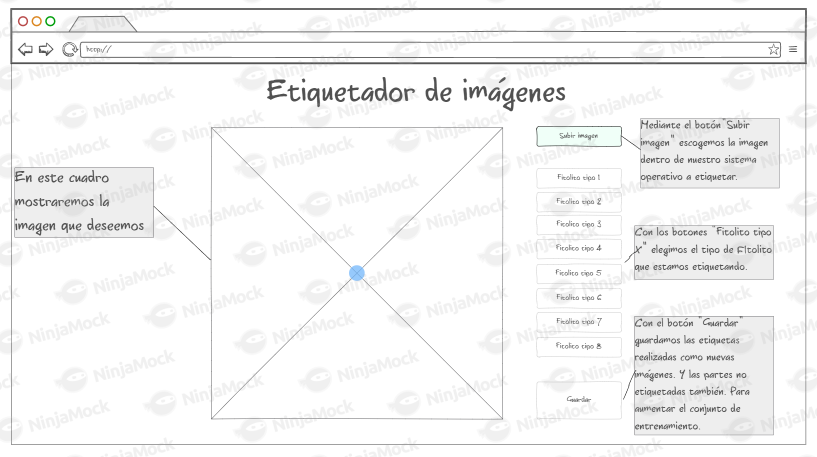
\includegraphics[width=0.99\textwidth]{protototipo_etiquetador_de_imagenes}
\caption{Prototipo del etiquetador de imágenes}
\label{fig:C.5.2}
\end{figure}

El resultado tras la implementación de este producto es el mostrado en la \ref{fig:C.5.3}. Obteniendo una interfaz muy similar a la prototipada en un principio. Pero añadiendo algún elemento más, para facilitar su uso por parte del usuario.

\begin{figure}[h]
\centering
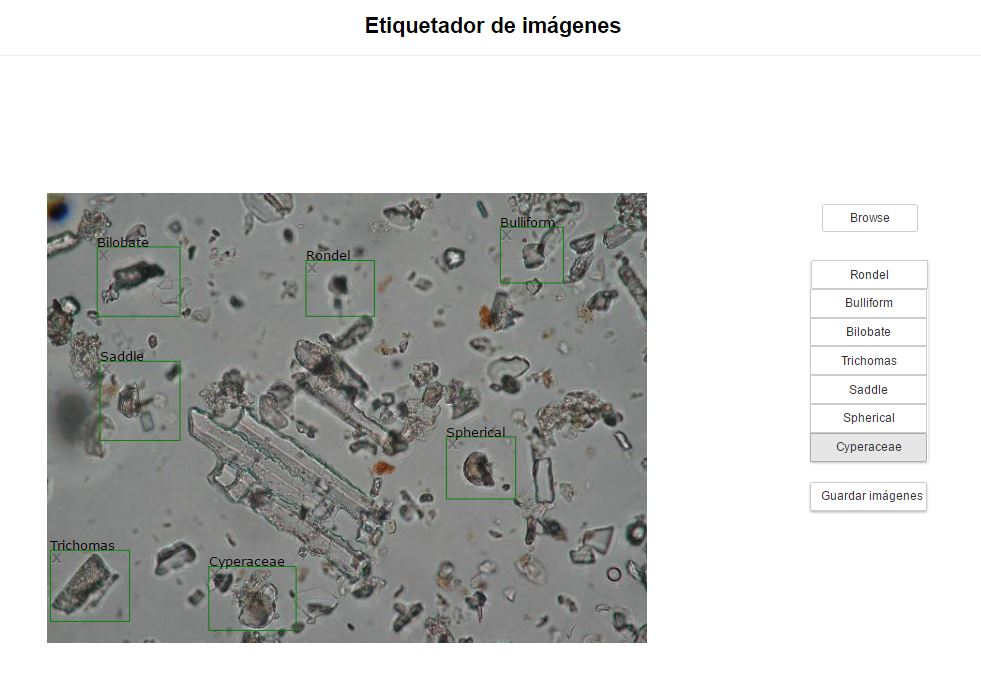
\includegraphics[width=0.99\textwidth]{etiquetador_de_imagenes_v1}
\caption{Etiquetador de imágenes}
\label{fig:C.5.3}
\end{figure}